We have seen that even problems with multiple dimensions of
flexibility, e.g., for the joint optimization of 
flexible node placement 
and replica selection, and even under capacity constraints (our problem
($\FP+\RS+\BW$), can be solved in polynomial time.
This section now points out fundamental
limitations in terms of computational tractability. In particular,
we will show that problems become NP-hard if
inter-connects have to be established ($\FP+\RS+\CC$ is proved
NP-hard in Section~\ref{ssec:fprscc}) or if multiple replicas
have to be assigned to a node ($\FP+\RS+\MA$ is proved
NP-hard in Section~\ref{ssec:fprsma}); both results hold
even in uncapacitated networks, and even in fat-trees consisting
of two levels only (e.g., in a datacenter \emph{pod}). Finally, we show that
some problems are NP-hard even if the number of replicas is only two
(Section~\ref{ssec:two}).

\subsection{Inter-connects are hard ($\FP+\RS+\CC$)}\label{ssec:fprscc}

We first prove that the joint optimization of node placement and replica selection
is NP-hard if an inter-connect has to be established between virtual machines.
In our terminology, this is the  $\FP+\RS+\CC$ problem.

The NP-hardness proof is by reduction from the \emph{set cover problem},
and in particular, from the set cover variant where all 
sets have cardinality exactly three. We will
refer to this problem by \emph{3-Set-Cover} or simply $\TSC$;
it is also NP-hard.

FIXME:There they say that 3HS in NP-complete:
\url{http://lcbb4.epfl.ch/reading/hitting\%20set/2003-niedermeierFPT3HS.pdf}
\url{http://www.sciencedirect.com/science/article/pii/S1570866703000091}

Formally, the input to $\TSC$ is a universe $U$, an integer $k$,
and a set of subsets
$S = \{ S_1, S_2, \ldots, S_n \}$ over $U$, where each subset is of 
cardinality three. The problem is to decide whether there
exists a set of subsets $S' \subset S$ of cardinality $k$, such that
every element in $U$ is covered.

\textbf{Construction.}
Given an instance of $\TSC$, we construct an instance of a
$\FP+\RS+\CC$ problem as follows. For each element
in the universe $U$, we construct a chunk; and for each 
subset $S_i$, we construct a gadget that contains
three replicas of chunks corresponding to the elements in the subset. 
We connect the gadgets in such a way that it is ensured
that subset $S_i$ is
chosen in $\TSC$ instance if and only if it contains three nodes. 
If each chunk is matched to a node, the entire universe
is covered. 


Concretely, let $I$ be an instance of $\TSC$. We will create an instance $I'$
for $\FP+\RS+\CC$ as follows: 
\begin{itemize}
\item We set the access cost $\CostTrans$ to a replica to a high value $W$. This will force
nodes to be collocated with the replica.
(For now, we can assume that $W=\infty$; a lower and sufficient bound will be given
in the appendix.)
\item The communication cost in the inter-connect is set to $\CostCom = 1$.
\item The number of nodes (virtual machines) is $\Vms = 3 \cdot k$.
\item We use a threshold $\Thr =  3 \cdot k + 3 \cdot 3 \cdot 2 \cdot (k - 1)$.
\end{itemize}

We construct a height-2 substrate tree 
as follows. For each $S_i$ we construct a gadget
consisting of an inner node (a router) and three leaves. Every gadget
contains three chunks, corresponding to the elements of $S_i$.

FIXME: The construction is illustrated in Figure~\ref{fig:fprscc}.

\textbf{Proof of correctness.}
Intuitively, in order to minimize embedding costs,
nodes should be placed on near-by replicas. We use the following
helper lemma. 
\begin{lemma}\label{lemma:helper}
In every valid solution $\Sol$ of $I'$ of cost $\leq \Thr$, each gadget
falls in one of two categories: 
$k$ gadgets have exactly
$3$ nodes, and $n-k$ gadgets remain empty.
\end{lemma}
\begin{proof}
Since $W=\infty$, nodes will always be placed
directly on chunks (the access network cost is zero). 
Moreover, since
$\Sol$ is valid, $|U|$ nodes are mapped
directly to the different chunk locations. 
Now, consider any pair of nodes communicating over the
inter-connect; due to our construction, the communication cost 
for each such pair is either 
2 hops (if they belong to the same gadget) or 4 hops (if they belong
to different gadgets). 
The lemma then follows from the observation that $\Thr$
is chosen such that it is never possible to distribute nodes
among more than $k$ gadgets, and that it is always strictly better to
have exactly 0 or 3 nodes per gadget, than any alternative distribution.
\end{proof}

\begin{theorem}
$\FP+\RS+\CC$ is NP-hard.
\end{theorem}
\begin{proof}
Let $I$ be an instance of $\TSC$ and let $I'$ be an instance of
$\FP+\RS+\CC$ constructed as described above.
We prove that $I'$ has solution of cost $\leq \Thr$ if ($\Rightarrow$) and only if
($\Leftarrow$)
$I$ has a solution of $k$.

($\Rightarrow$) In order to compute a solution
for $I'$ given a solution for $I$, we proceed as follows.
Given a covering set $S = \{S_1, S_2, \ldots, S_k\}$, we place three nodes in each gadget that
corresponds to every subset. Nodes are matched to chunks 
as follows: we traverse nodes one by one, and if the node is
located at a chunk which has not been taken into account yet,
the chunk is assigned to this node; otherwise 
the node is set to idle. 
The solution has the following cost: 
(1) the communication cost inside a gadget is $2 \cdot {3 \choose 2}$,
  as every pair contributes two hops;
  (2) the communication cost from each gadget to all other gadgets is $4
  \cdot 3 \cdot 3 \cdot (k - 1) / 2$, where the factor $2$ is 
  for the 
  communication over $4$ hops, the factor $3$
  corresponds to the number of nodes per gadget, and 
  $3 \cdot (k-1)$ is the number of nodes in remote gadgets; 
  as we count each pair twice, we need to divide by two in the end.
Summing up over all $k$ gadgets, we get exactly $\Thr$.

($\Leftarrow$) Given a solution for $I'$,
we can exploit Lemma~\ref{lemma:helper} to construct a solution for $I$.
We know that in any solution of cost at most $\Thr$,
$k$ gadgets contain exactly 3 nodes. These gadgets correspond to a valid
set cover of size $k$: every
chunk and hence element in the universe, is covered. 
\end{proof}

\subsection{Multi-Assignments are hard ($\FP+\RS+\MA$)}\label{ssec:fprsma}

Next, we show the hardness of a problem variant without inter-connect,
but where nodes are assigned multiple chunks, namely the $\FP+\RS+\MA$
problem.
The reduction is from three-dimensional matchings, a generalization of bipartite matchings
to 3-uniform hypergraphs, henceforth called
$\TDM$.~\cite{3dmatch} 

$\TDM$ is defined as follows. We are given three finite and disjoint sets $X$, $Y$, and $Z$, 
as well as a subset of triples $T\subset X \times Y \times Z$.
Set $M \subseteq T$ is a 3-dimensional matching if and only if, 
for any two distinct triples $(x_1, y_1, z_1) \in M$ and $(x_2, y_2, z_2) \in M$,
it holds that $x_1\neq x_2$, $y_1\neq y_2$, and $z_1\neq z_2$. Our goal is to 
maximize the cardinality of $M$. 

\textbf{Construction.}
Given an instance $I$ of $\TDM$, we construct an instance $I'$ of
$\FP+\RS+\MA$ as follows:
\begin{itemize}
\item We construct a tree consisting of gadgets, where each gadget corresponds to a triple.
\item Chunks correspond to elements in $X$, $Y$ and $Z$
\item $|X| = |Y| = |Z| = k$
\item we set $\CostTrans=1$
\item we set m to 3
\item we set number of VMs to $k$
\item we set $\Thr=2 \cdot 2 \cdot k$
\item each gadget consists of 3 leaves and parent; in leaves there are
  chunks that correspond to elements of a triple
\end{itemize}

\textbf{Correctness.}

\begin{theorem}
$\FP+\RS+\MA$ is NP-hard.
\end{theorem}
\begin{proof}
Let $I$ be an instance of $\TDM$ and let $I'$ be an instance of
$\FP+\RS+\MA$ constructed as described above.
We prove that $I'$ has solution of cost $\leq \Thr$ if ($\Rightarrow$) and only if
($\Leftarrow$)
$I$ has a matching of size $k$.

($\Rightarrow$) Let us take a solution to $\TDM$. We spawn VM in every
gadget that corresponds to chosen triples. We match every chunk in a
gadget to machine in this gadget (only for chosen ones). Solution has
cost exactly $\Thr$.

($\Leftarrow$) Let's take solution to $VC$ instance of cost $\leq \Thr$. We
chose triples that correspond to gadgets where were VMs. Everything
was processed, therefore every element of X,Y and Z is matched.
\end{proof}


\subsection{Two replicas are hard ($\FP+\RS(2)+\BW$)}\label{ssec:two}

Our results so far indicate that dealing with replication can be challenging.
However, all our hardness proofs concerned scenarios with three replicas,
which raises the question whether the problems can be solved in polynomial time
with a replication factor of two only. (Similarly, say, to the $ZSAT$ problem
which is tractable in contrast to $\TSAT$.)

In the following, we show that this is not the case: the problem remains
NP-hard, at least in the capacitated network. 

The proof is by reduction from $\TSAT$. Given a formula $\Psi$ in
conjunctive normal form, we construct a problem instance and substrate tree 
$T_{\Psi}$ using two types of gadgets: gadgets for variables and
gadgets for clauses. Nota bene: 
unlike in the previous proofs, for every clause we will create three chunk types instead of just one.

\textbf{Construction.}
We distribute chunks among servers as follows. First, 
similarly to the previous proofs with three replicas, we put clause chunks in
variable gadgets; however, now we place distinct chunks instead of
three copies of the same chunk. Second, we place three chunks that
correspond to clauses in all three leaves of their clause gadgets. 
Thus, in total, $6 \cdot c$ variable chunks are mapped.
We will consider a setting where $cv + 2c$ nodes need to be mapped. Our intention is that in
every variable gadget, there will be $c$ nodes,
 and in every of clause
gadgets there will be two nodes.

The available bandwidth of the top edge of each variable gadget is set to
$ bw(v) = 3  \cdot  3  \cdot  (3  \cdot  (v - 1) + 2  \cdot  c) $.
The first factor is the tree distance which is 6 divided by 2 (as
we count each pair twice). The second factor is
the number of nodes to be placed in every variable gadget. 
So the first term of the 
sum is three times the number of outer variable gadgets,
and the second term is the
number of nodes in each of the $c$ clause gadgets.

The available bandwidth for the top edge of each clause gadget is set to
$ bw(c) = 3  \cdot  2  \cdot  (2  \cdot  (c - 1) + 3  \cdot  v) $.

\textbf{Proof of correctness.}
We first prove the following helper lemma.
\begin{lemma}
Every valid solution to $\FP+\RS(2)+\BW$
with cost at most $\Thr$ has the property that
there are exactly $c$ nodes in each of the $v$ variable gadgets
and exactly two nodes in each of the $c$ clause gadgets.
\end{lemma}
\begin{proof}
The claim is due to the bandwidth constraints. We have to take into
consideration the following communication paths: 
communication to clause gadgets and 
communication to
other variable gadgets. 
In every valid solution of cost at most $\Thr$ we have exactly
$c$ VMs in each variable gadget and $2$ VMs in each clause gadget.
\end{proof}

\begin{theorem}
$\FP+\RS(2)+\BW$ is NP-hard.
\end{theorem}
\begin{proof}
We show that $\FP+\RS(2)+\BW$ has a solution of cost $\leq
  \Thr$ if and only if $\Formula \in \TSAT$.
  
($\Rightarrow$) If we have a positive valuation of $\Formula$, we fill variable gadgets with nodes like in
the proofs before. Then we fill $2 \cdot c$ nodes as follows:
\begin{itemize}
\item If the first literal satisfied the clause, we put two nodes in the second and
third leaf of the corresponding clause gadget.
\item If the first literal does not satisfy the clause, we put two VMs in first
and second leaf of clause gadget
\end{itemize}

We assign chunks to nodes as follows:
\begin{itemize}
\item Chunk $c_i^1$ is matched to the node which is located in a variable gadget; there
must be one, as the valuation satisfies the formula.
\item Chunks $c_i^2$ and $c_i^3$ are matched to nodes which are
located in clause
gadgets; there exist minimal-cost solutions where VMs sit there
\end{itemize}

Thus, we have produced a feasible solution of cost $\Thr$, as there are no
access and inter-connect costs. 

($\Leftarrow$) 
Let's take any solution $\Sol$ to $\FP+\RS(2)+\BW$ of cost $\leq \Thr$.
Then we can compute a positive valuation as follows:
\begin{itemize}
\item We set $\Val(v) = \top$ iff there lies VM on first leaf on positive side of $v$ gadget in $\Sol$
\item Otherwise, we set $\Val(v) = \bot$.
\end{itemize}

The theorem now follows from the following two additional lemmas.
\begin{lemma}
For every clause there exists a node in a variable gadget that processes one of
  three chunks that correspond to that clause.
\end{lemma}
\begin{proof}
 Each of the three chunks that correspond to every clause,
 is assigned a collocated node. 
 At least one of those three nodes is not idle in a variable gadget;
otherwise, those two VMs in clause gadgets would not suffice in
satisfying all chunk types.\end{proof}

Observation. It might happen that in $SOL$ $2$ VMs in
clause variables are idle, and $3$ VMs in variable gadgets are
processing those $3$ chunk types, then we can take arbitrary in the rest
of the proof.

\begin{lemma}
$\Val$ satisfies $\Formula$.
\end{lemma}
\begin{proof}
Let's take the matching $M$ of $\Sol$, and let's take an arbitrary clause of
$\Formula$ and its $3$ chunk types: $c_i^1, c_i^2, c_i^3$. Let's name machines corresponding to them
to $vm_i^1, vm_i^2, vm_i^3$. Two of those lie in clause gadgets. Let's
take the chunk type that was processed in variable
gadgets and look at where it was processed. Look how was labeled the
leaf the VM lies. In our valuation Val we set this literal to have
value True. Therefore the clause is satisfied.
\end{proof}
\end{proof}

\subsection{Images}

\begin{figure}[htbp]
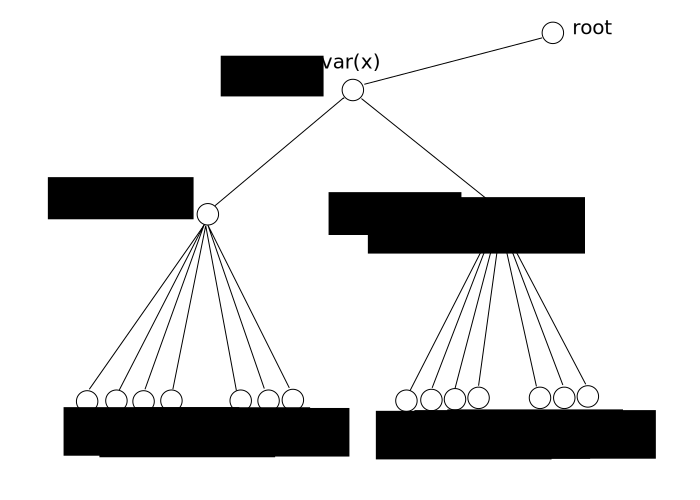
\includegraphics[width = \columnwidth]{figs/gadget-no-bw}
\end{figure}


\begin{figure}[htbp]
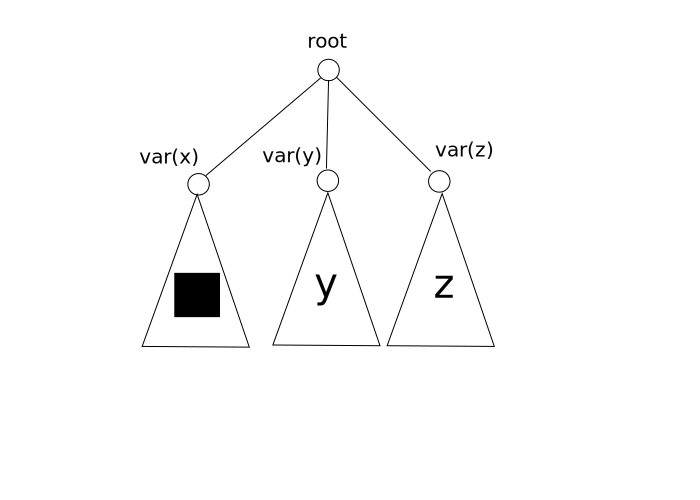
\includegraphics[width = \columnwidth]{figs/vc-instance}
\end{figure}


\begin{figure}[htbp]
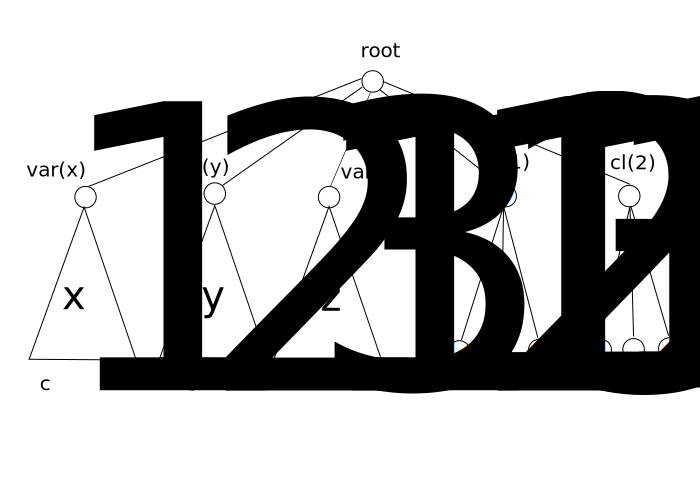
\includegraphics[width = \columnwidth]{figs/vc-instance-r2}
\end{figure}


\begin{figure}[htbp]
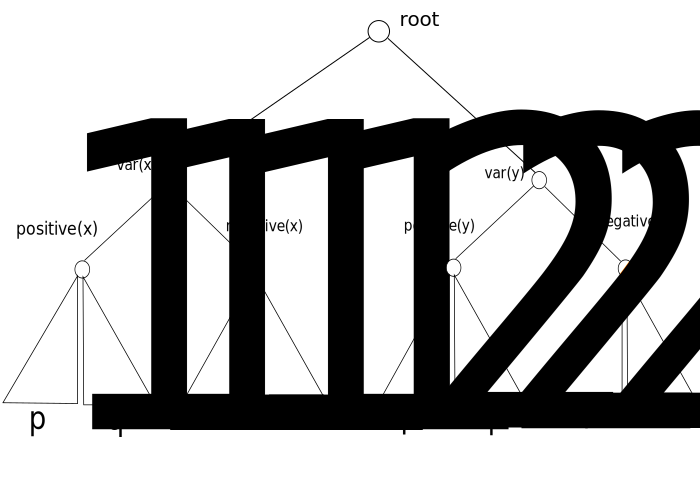
\includegraphics[width = \columnwidth]{figs/lemma-two-gadgets}
\end{figure}


\begin{figure}[htbp]
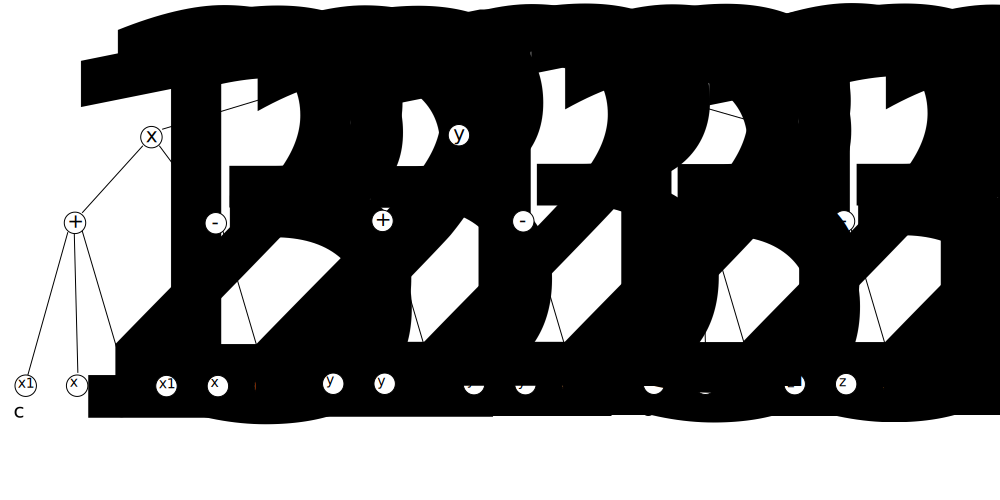
\includegraphics[width = \columnwidth]{figs/formula-example}
\end{figure}

